
%(BEGIN_QUESTION)
% Copyright 2011, Tony R. Kuphaldt, released under the Creative Commons Attribution License (v 1.0)
% This means you may do almost anything with this work of mine, so long as you give me proper credit

The following screen capture shows the configuration window for an HMI panel, providing serial communication parameters for it to exchange data with a Modbus device:

$$\includegraphics[width=15.5cm]{i00718x01.eps}$$

Identify the purpose for the ``Control RTS'' and ``Require CTS'' parameters, both of which happen to be de-activated (set to ``No'').

\vskip 50pt

Two options exist for Modbus Register Write function codes: 06 and 16.  Likewise, two options exist for Modbus Coil Write function codes: 05 and 15.  Explain the difference between each option, and why one setting might be more useful than the other.

\vfil 

\underbar{file i00718}
\eject
%(END_QUESTION)





%(BEGIN_ANSWER)

This is a graded question -- no answers or hints given!

%(END_ANSWER)





%(BEGIN_NOTES)

``Control RTS'' and ``Require CTS'' refers to {\it handshaking} signals optionally exchanged between the HMI and the serial device.  ``Request To Send'' and ``Clear To Send'' signals ensure the receiving device (the Modbus device in this case) is ready to receive a transmission (from the HMI panel).  Waiting to send and receive these handshaking signals takes extra time, which is why they are turned off by default.

\vskip 10pt

Modbus codes 15 and 16 allow for {\it multiple} coils and registers to be written, while codes 05 and 06 only allow for {\it single} registers and coils to be written at a time.  If many registers/coils need to be written at a time (to save communications time), it is best to select codes 15 and 16 rather than 05 and 06.

%(END_NOTES)


